% !TeX program = lualatex

\documentclass[a4paper]{report}

% ===== PACKAGES FOR VIETNAMESE & FONTS =====
\usepackage{fontspec}
\setmainfont{Times New Roman}

% ===== PAGE SETUP =====
\usepackage[
    top=3cm,
    bottom=3.5cm,
    left=3.5cm,
    right=2cm
]{geometry}

% ===== LINE SPACING =====
\usepackage{setspace}
\onehalfspacing

% ===== FORMATTING =====
\usepackage{fancyhdr}
\usepackage{tocloft}
\usepackage{graphicx}
\usepackage{float}
\usepackage{hyperref}
\usepackage{amsmath}
\usepackage{amssymb}

% ===== CHAPTER FORMATTING =====
\usepackage{titlesec}
\titleformat{\chapter}
  {\normalfont\huge\bfseries} % font giữ nguyên
  {Chương \thechapter}       % phần label
  {0.5em}                     % khoảng cách
  {}                          % trước title
\titlespacing*{\chapter}{0pt}{-0.2in}{0.3in}



% ===== VIETNAMESE LABELS =====
\renewcommand{\figurename}{Hình}
\renewcommand{\contentsname}{Mục lục}

% ===== TABLE OF CONTENTS FORMATTING =====
\renewcommand{\cftchapleader}{\cftdotfill{\cftdotsep}}
\renewcommand{\cftsecnumwidth}{3em}
\renewcommand{\cftsubsecnumwidth}{3em}

% ===== HEADER & FOOTER =====
\pagestyle{fancy}
\fancyhf{}
\fancyfoot[C]{\thepage}
\renewcommand{\headrulewidth}{0pt}

% ===== CUSTOM COMMANDS =====
\newcommand{\toc}{\tableofcontents\newpage}

% ===== DOCUMENT =====
\begin{document}

% ===== FONT SIZE 13pt =====
\fontsize{13pt}{15.6pt}\selectfont

% ===== NO PAGE NUMBERING FOR FRONT MATTER =====
\pagenumbering{gobble}

% ===== TITLE PAGE =====
\begin{titlepage}
    \centering
    \vspace*{1cm}

    {\Large \bfseries ĐẠI HỌC QUỐC GIA TP. HỒ CHÍ MINH}

    {\Large \bfseries TRƯỜNG ĐẠI HỌC CÔNG NGHỆ THÔNG TIN}

    {\Large \bfseries KHOA CÔNG NGHỆ PHẦN MỀM}

    \vspace{3cm}

    {\Large \bfseries ĐỒ ÁN 1}

    \vspace{1cm}

    {\Large \bfseries TÌM HIỂU CÔNG NGHỆ MCP ĐỂ BUILD RICH CONTEXT AI APP}

    \vspace{3cm}

    {\large \bfseries GV HƯỚNG DẪN:}

    {\large Th.S Nguyễn Công Hoan}

    \vspace{1cm}

    {\large \bfseries SV THỰC HIỆN:}

    {\large Quách Gia Kiệt - 23520819} \\
    {\large Nguyễn Tuấn Kiệt - 23520815}

    \vspace{4cm}

    {\large TP. HỒ CHÍ MINH, 2025}
\end{titlepage}

% ===== ACKNOWLEDGMENTS =====
\chapter*{}
\begin{center}
    \Large\bfseries LỜI CẢM ƠN
\end{center}
\addcontentsline{toc}{chapter}{Lời cảm ơn}

Nhóm chúng em xin gửi lời cảm ơn và lòng biết ơn sâu sắc nhất tới thầy
Nguyễn Công Hoan, giảng viên hướng dẫn cho nhóm. Thầy đã luôn nhiệt tình, đồng
hành, hỗ trợ và giúp đỡ chúng em trong suốt quá trình thực hiện Đồ án 1.

Trong thời gian một học kỳ thực hiện đề tài, nhóm chúng em đã vận dụng
những kiến thức nền tảng đã tích lũy đồng thời kết hợp với việc học hỏi và nghiên
cứu những kiến thức mới, và đặc biệt là những kiến thức từ lý thuyết đến thực hành
mà thầy đã nhiệt huyết giảng dạy cho chúng em. Từ đó, nhóm chúng em vận dụng tối
đa những gì đã thu thập được để hoàn thành một báo cáo đồ án và seminar tốt nhất.

Trong quá trình thực hiện đồ án này, với kinh nghiệm và thời gian có
hạn, nhóm không tránh khỏi được sai sót, chúng em kính mong nhận được sự góp ý,
hướng dẫn của thầy để có thể hoàn thiện đồ án hơn nữa, cũng như là hành trang để
nhóm chúng em thực hiện tiếp các đề tài khác trong tương lai.

Nhóm em xin chân thành cảm ơn thầy!

\vspace{1cm}

\begin{flushright}
    Nhóm sinh viên thực hiện\\
    Quách Gia Kiệt - Nguyễn Tuấn Kiệt
\end{flushright}

\newpage

% ===== TABLE OF CONTENTS =====
\tableofcontents
\newpage

% ===== ABSTRACT =====
\chapter*{}
\begin{center}
    \Large\bfseries TÓM TẮT ĐỒ ÁN
\end{center}
\addcontentsline{toc}{chapter}{Tóm tắt đồ án}

% ===== START PAGE NUMBERING FROM HERE =====
\pagenumbering{arabic}
\setcounter{page}{1}
\pagestyle{fancy}

% Tóm tắt đồ án (1-2 trang)
% Trình bày tóm tắt vấn đề nghiên cứu, các hướng tiếp cận, cách giải quyết vấn đề và một số kết quả đạt được

\section*{Vấn đề nghiên cứu}

Sinh viên Đại học Công nghệ Thông tin (UIT) phải quản lý nhiều thông tin học vụ phức tạp từ các hệ thống
khác nhau: tra cứu quy định về điều kiện tốt nghiệp, yêu cầu môn học theo ngành, xem lịch học và lịch thi,
kiểm tra điểm số từ hệ thống DAA, tìm tài liệu học. Các thông tin này không được tập trung ở một nơi mà
phân tán trên nhiều nền tảng khác nhau. Để tìm kiếm thông tin, sinh viên phải truy cập nhiều trang web, ghi nhớ các điều khoản quy định, hoặc hỏi cán bộ hỗ trợ. Quá trình
này tốn thời gian, dễ bị nhầm lẫn, và không hiệu quả.

Để giải quyết vấn đề này, đề tài xây dựng một AI agent để hỗ trợ sinh viên
trong việc quản lý và tra cứu thông tin học vụ. AI agent có khả năng hiểu các câu hỏi tự nhiên
từ sinh viên, suy luận logic, gọi các công cụ thích hợp, và cung cấp câu trả lời chính xác từ các nguồn dữ liệu một cách nhanh chóng.

\section*{Cách giải quyết vấn đề}

Để xây dựng AI agent hỗ trợ sinh viên, đề tài sử dụng một kiến trúc kết hợp ba thành phần chính:
Retrieval-Augmented Generation (RAG), Model Context Protocol (MCP), và LangGraph để orchestrate agent logic.

Cụ thể, RAG được sử dụng để xây dựng knowledge base từ các tài liệu quy định và chương trình đào tạo,
cho phép agent tìm kiếm và trích xuất thông tin chính xác. MCP được dùng để tích hợp các công cụ bên
ngoài như DAA portal (lấy điểm, lịch thi) và knowledge base retrieval. LangGraph được dùng để thiết kế
AI agent theo ReAct pattern (Reasoning + Acting) có khả năng suy luận, chọn tools phù hợp, và xử lý multi-step queries.

Ba thành phần này kết hợp với nhau để tạo thành một AI agent hoàn chỉnh: khi nhận câu hỏi từ người dùng,
agent suy luận xem cần gọi tools nào (retrieval từ knowledge base hoặc scraping từ DAA), thực thi các tool
calls đó, nhận kết quả, và sinh ra câu trả lời hoàn chỉnh cho sinh viên.

\section*{Kết quả đạt được}

Đề tài đã xây dựng một AI agent như một proof-of-concept để hỗ trợ sinh viên UIT quản lý và tra cứu thông tin học vụ.
AI agent có khả năng trả lời các câu hỏi về quy định đào tạo, chương trình học, và có thể tự động lấy thông tin
như lịch thi, điểm số, thời khóa biểu từ các hệ thống bên ngoài. Hệ thống được tích hợp vào một nền tảng web
cho phép sinh viên tương tác với agent. Tuy nhiên, hiện tại agent còn những hạn chế như độ chính xác truy vấn chưa cao,
số lượng tính năng còn hạn chế, và cần các bước tối ưu hóa thêm.

Bất chấp những hạn chế này, kết quả đạt được chứng minh rằng kiến trúc tích hợp RAG, MCP, và LangGraph có khả năng
hoạt động hiệu quả trong việc xây dựng AI agent hỗ trợ học vụ. Nền tảng này mở ra các cơ hội để nâng cấp thêm độ chính xác,
mở rộng tính năng, và triển khai rộng rãi cho các trường đại học khác trong tương lai.


\newpage

% ===== MAIN CHAPTERS =====
\chapter{Mở đầu}

% Trình bày lí do chọn đề tài, mục đích, đối tượng và phạm vi nghiên cứu

\section{Lý do chọn đề tài}

Sinh viên Đại học Công nghệ Thông tin (UIT) phải quản lý một lượng lớn thông tin học vụ từ nhiều hệ thống khác nhau.
Các thông tin này bao gồm quy định về điều kiện tốt nghiệp, yêu cầu môn học theo ngành, lịch học, lịch thi, điểm số,
và các tài liệu học tập. Tuy nhiên, các thông tin này không được tập trung ở một nơi mà phân tán trên nhiều nền tảng
và hệ thống khác nhau như DAA portal, website khoa, trang thông báo, v.v.

Để tìm kiếm thông tin, sinh viên phải truy cập nhiều trang web, ghi nhớ các quy định, hoặc liên hệ với cán bộ hỗ trợ.
Quá trình này tốn thời gian, dễ dẫn đến nhầm lẫn, và không hiệu quả. Nhận thấy vấn đề này, đề tài quyết định xây dựng
một AI agent có khả năng trả lời các câu hỏi tự nhiên từ sinh viên, giúp họ nhanh chóng truy cập thông tin học vụ một cách
dễ dàng và chính xác.

\section{Mục đích}

Đề tài có mục đích xây dựng một AI agent có khả năng hỗ trợ sinh viên UIT trong việc quản lý và tra cứu thông tin học vụ.
Cụ thể, AI agent sẽ có khả năng hiểu các câu hỏi tự nhiên từ sinh viên, suy luận logic để xác định loại thông tin cần tìm,
gọi các công cụ thích hợp (truy vấn knowledge base hoặc lấy dữ liệu từ DAA portal), và cung cấp câu trả lời chính xác
một cách nhanh chóng.

Bên cạnh đó, đề tài cũng nhằm chứng minh khả năng tích hợp và ứng dụng thực tế các công nghệ AI hiện đại như Retrieval-Augmented
Generation (RAG), Model Context Protocol (MCP), và LangGraph trong việc xây dựng các ứng dụng phục vụ người dùng cuối.

\section{Đối tượng nghiên cứu}

Đối tượng nghiên cứu của đề tài là các sinh viên Đại học Công nghệ Thông tin (UIT), đặc biệt là những sinh viên
cần tra cứu thông tin học vụ như quy định tốt nghiệp, yêu cầu môn học, lịch thi, điểm số, thời khóa biểu, và tài liệu
học tập. Ngoài ra, đề tài cũng tập trung vào việc phát triển một AI agent có khả năng hiểu và xử lý các câu hỏi tự nhiên
từ sinh viên, làm nền tảng để các ứng dụng tương tự có thể áp dụng cho các trường đại học khác.

\section{Phạm vi nghiên cứu}

Phạm vi nghiên cứu của đề tài bao gồm:

\textbf{Về mặt chức năng:} AI agent được xây dựng để trả lời các câu hỏi liên quan đến (1) quy định đào tạo và tốt nghiệp
của UIT, (2) yêu cầu môn học theo từng ngành học, (3) thông tin lịch thi và lịch học, (4) điểm số và kết quả học tập
lấy từ DAA portal. Đề tài không bao gồm các chức năng khác như đăng ký môn học, xin học lại, hay các dịch vụ hành chính
khác.

\textbf{Về mặt công nghệ:} Đề tài tập trung vào việc tích hợp ba thành phần chính: Retrieval-Augmented Generation (RAG)
cho knowledge base, Model Context Protocol (MCP) cho tích hợp công cụ, và LangGraph cho orchestration logic của AI agent.
Phạm vi không bao gồm việc huấn luyện mô hình LLM từ đầu, mà sử dụng các mô hình có sẵn như Claude hoặc các mô hình mã
nguồn mở khác.

\textbf{Về mặt triển khai:} Hệ thống được thiết kế cho môi trường UIT với dữ liệu và hệ thống của trường này. Tuy nhiên,
kiến trúc được thiết kế để có thể mở rộng cho các trường đại học khác trong tương lai.

\include{chapters/02_theory}
\chapter{Kết quả triển khai}

% Chi tiết quá trình xây dựng hệ thống, các kết quả đạt được, và minh họa bằng diagram, screenshot

\section{Tổng quan kiến trúc hệ thống}

\subsection{Kiến trúc tổng thể}

Hệ thống được thiết kế theo kiến trúc modular, gồm 5 thành phần chính hoạt động cùng nhau để hỗ trợ sinh viên truy vấn thông tin học vụ:

\begin{enumerate}
    \item \textbf{Knowledge Base (RAG System):} Tập hợp các tài liệu đã được xử lý và lưu trữ dưới dạng vector embeddings trong ChromaDB. Hệ thống này giữ các tài liệu quy định, chương trình đào tạo của UIT, cho phép tìm kiếm semantic để lấy thông tin liên quan đến truy vấn của sinh viên.

    \item \textbf{AI Agent (LangGraph):} Thành phần trung tâm orchestrate toàn bộ quy trình. Agent sử dụng ReAct pattern để suy luận về công cụ cần gọi, gọi MCP tools, nhận kết quả, và tổng hợp thông tin để sinh ra câu trả lời hoàn chỉnh cho sinh viên.

    \item \textbf{MCP Server:} Cung cấp các công cụ (tools) mà agent có thể sử dụng. Các tools chính bao gồm: Knowledge Base Retrieval (truy vấn vector store để lấy tài liệu), DAA Integration (kết nối với hệ thống học vụ để lấy dữ liệu cá nhân sinh viên như lịch thi, điểm số), và các tools xử lý dữ liệu khác.

    \item \textbf{API Gateway:} Cầu nối giữa giao diện người dùng (frontend) và hệ thống backend. Nó tiếp nhận các yêu cầu từ người dùng, chuyển tiếp đến agent, và trả về kết quả cho người dùng.

    \item \textbf{Giao diện người dùng (UI):} Bao gồm 2 phần: Web frontend (giao diện web trên browser) và Browser extension (tiện ích mở rộng cho trình duyệt). Hai giao diện này cho phép sinh viên tương tác với agent một cách thuận tiện.
\end{enumerate}

Quy trình hoạt động tổng thể: Sinh viên đặt câu hỏi thông qua giao diện → API Gateway chuyển tiếp → Agent nhận câu hỏi, suy luận, gọi MCP tools → MCP Server thực thi công cụ (truy vấn knowledge base hoặc DAA) → Agent nhận kết quả, tổng hợp, và sinh ra câu trả lời → Trả về cho người dùng qua API Gateway.

\begin{figure}[h]
    \centering
    \includegraphics[width=\textwidth]{images/architecture/system_architecture.png}
    \caption{Kiến trúc tổng thể của hệ thống}
    \label{fig:system_architecture}
\end{figure}

\subsection{Tech stack}

Hệ thống được xây dựng trên nền tảng công nghệ đa dạng, kết hợp các framework và công cụ hiện đại để tạo thành một kiến trúc microservices hoàn chỉnh.

Về backend, hệ thống sử dụng hai ngôn ngữ chính: Go và Python. API Gateway được phát triển bằng Go với framework Gin, cung cấp hiệu năng cao cho việc xử lý HTTP requests và giao tiếp với frontend. AI Agent và MCP Server được xây dựng bằng Python, tận dụng hệ sinh thái phong phú của Python trong lĩnh vực AI. Agent sử dụng LangGraph để orchestrate luồng xử lý theo ReAct pattern, trong khi MCP Server dựa trên FastMCP framework để expose các tools theo chuẩn Model Context Protocol. Knowledge Builder là một CLI tool Python dùng để xây dựng knowledge base offline.

Về mặt AI và machine learning, hệ thống tích hợp các mô hình ngôn ngữ lớn thông qua LangChain, hỗ trợ cả OpenAI GPT và Google Gemini. Hệ thống RAG được xây dựng trên LlamaIndex framework, cung cấp các công cụ cho indexing, retrieval, và query processing. Vector embeddings được tạo bằng OpenAI text-embedding-3-small model. Đặc biệt, hệ thống sử dụng ViRanker - một reranking model tiếng Việt - chạy trên Modal serverless GPU để cải thiện độ chính xác của retrieval.

Hệ thống sử dụng bốn loại database khác nhau, mỗi loại phục vụ một mục đích riêng: MongoDB lưu trữ chat sessions và messages để hiển thị trên giao diện; PostgreSQL được dùng làm checkpointer cho LangGraph, lưu trạng thái của agent; Redis cache các credentials và dữ liệu tạm thời; ChromaDB là vector database lưu trữ embeddings của knowledge base.

Giao diện người dùng bao gồm hai phần: Web frontend được phát triển bằng React với Vite làm build tool và Tailwind CSS cho styling; Browser extension được xây dựng bằng Svelte, có nhiệm vụ đồng bộ cookies từ DAA portal lên Redis.

Về infrastructure, các thành phần được containerized bằng Docker và orchestrate bằng Docker Compose. Hệ thống giao tiếp nội bộ thông qua nhiều protocol: gRPC cho communication giữa API Gateway và Agent, HTTP/REST cho frontend và API Gateway, MCP over HTTP cho Agent và MCP Server.

\section{RAG}

\subsection{Indexing}

Quá trình indexing là bước đầu tiên để xây dựng knowledge base, nhằm chuyển đổi các tài liệu thô (PDF, DOCX) thành dạng vector embeddings có thể tìm kiếm được. Hệ thống sử dụng một pipeline gồm ba giai đoạn chính: thu thập dữ liệu, xử lý tài liệu, và vector indexing.

Giai đoạn đầu tiên là thu thập dữ liệu từ hai nguồn. Nguồn thứ nhất là các tài liệu được thu thập thủ công từ website UIT, bao gồm các quy định, chính sách học vụ, và chương trình đào tạo. Nguồn thứ hai là web scraping tự động để lấy các tài liệu mới được cập nhật. Dữ liệu thô được lưu vào thư mục tạm thời để chuẩn bị cho bước xử lý.

Giai đoạn thứ hai là xử lý tài liệu, bao gồm ba bước chính. Đầu tiên, các file PDF và DOCX được parse thành định dạng Markdown sử dụng LlamaParse - một parser dựa trên LLM có khả năng hiểu cấu trúc tài liệu tốt hơn các parser truyền thống. Tiếp theo, nội dung được làm sạch để loại bỏ các thành phần không cần thiết như header, footer, navigation. Cuối cùng, metadata của từng tài liệu được tạo tự động bằng LLM, bao gồm các thông tin như document ID, title, category, year, và các trường đặc thù cho từng loại tài liệu (ví dụ: effective\_date cho quy định, major và program\_type cho chương trình đào tạo).

Giai đoạn cuối cùng là vector indexing. Các tài liệu đã xử lý được chia nhỏ thành chunks theo một chiến lược được thiết kế riêng cho văn bản tiếng Việt và cấu trúc quy định của UIT. Hệ thống có khả năng nhận diện các pattern đặc trưng của quy định như "CHƯƠNG", "Điều", "Khoản", "Mục", và giữ nguyên hierarchy khi chia nhỏ tài liệu. Mỗi chunk được thêm context bao gồm document metadata và hierarchy path để cải thiện độ chính xác khi retrieval. Sau đó, các chunks được convert thành vector embeddings bằng OpenAI text-embedding-3-small model và lưu vào ChromaDB. ChromaDB tổ chức dữ liệu thành các collections riêng biệt cho từng category (regulation, curriculum), giúp tối ưu hóa tốc độ tìm kiếm.

\begin{figure}[H]
    \centering
    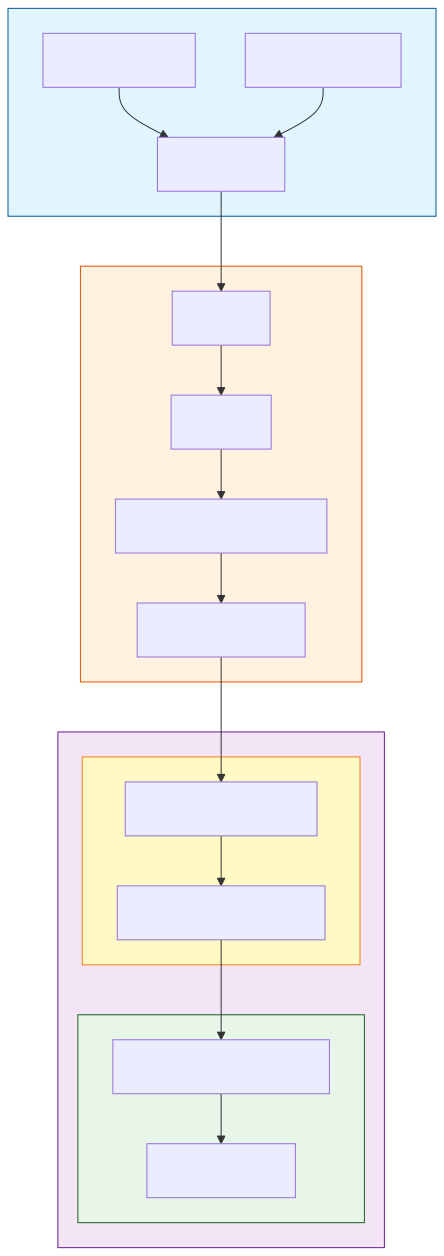
\includegraphics[width=\textwidth]{images/rag/indexing.png}
    \caption{Pipeline xây dựng knowledge base (indexing)}
    \label{fig:indexing_pipeline}
\end{figure}

\subsection{Retrieval Engine}

Retrieval engine là thành phần chịu trách nhiệm tìm kiếm và trả về các chunks liên quan nhất từ knowledge base khi nhận được query từ agent. Quá trình retrieval được thiết kế để tối ưu hóa độ chính xác thông qua kết hợp semantic search và reranking.

Khi một query được gửi tới, bước đầu tiên là chuyển đổi query thành vector embedding sử dụng cùng model đã dùng trong quá trình indexing (OpenAI text-embedding-3-small). Điều này đảm bảo rằng query và documents nằm trong cùng một không gian vector, cho phép tính toán độ tương đồng semantic một cách chính xác.

Tiếp theo, hệ thống thực hiện semantic search trên ChromaDB để tìm các chunks có embedding gần nhất với query embedding. ChromaDB sử dụng thuật toán approximate nearest neighbor search để nhanh chóng tìm ra top-K candidates (thường là 20 chunks). Quá trình này dựa trên cosine similarity giữa các vectors.

Để cải thiện độ chính xác, các candidates được gửi qua một bước reranking sử dụng ViRanker - một model reranking được huấn luyện trên tiếng Việt. ViRanker được deploy trên Modal serverless GPU, nhận query và danh sách candidates, sau đó tính toán relevance score chi tiết hơn cho từng candidate. Model này có khả năng hiểu ngữ cảnh tốt hơn simple vector similarity, giúp xếp hạng lại các kết quả chính xác hơn.

Sau khi có scores từ reranker, hệ thống áp dụng hai bước lọc. Đầu tiên là lọc theo threshold score (thường là 0.25) để loại bỏ các kết quả có độ liên quan quá thấp. Thứ hai là program filter - một cơ chế đặc biệt để tránh nhầm lẫn giữa các ngành đào tạo khác nhau khi query về chương trình học. Cuối cùng, top-3 chunks có score cao nhất được trả về cho agent kèm theo metadata đầy đủ. Agent sử dụng các chunks này làm context để sinh ra câu trả lời cho sinh viên.

\begin{figure}[H]
    \centering
    \includegraphics[width=0.7\textwidth]{images/rag/retrieval.png}
    \caption{Quy trình retrieval từ knowledge base}
    \label{fig:retrieval_pipeline}
\end{figure}

\subsection{Kết quả}

Hệ thống RAG đã được xây dựng với knowledge base bao gồm hai categories chính: quy định (regulation) và chương trình đào tạo (curriculum). Các tài liệu đã được xử lý, chia nhỏ thành chunks, và lưu trữ dưới dạng vector embeddings trong ChromaDB.

Pipeline indexing hoạt động cơ bản, có khả năng xử lý các tài liệu PDF và DOCX nhờ LlamaParse. Việc tự động generate metadata bằng LLM giúp tiết kiệm thời gian. Chiến lược chunking được thiết kế cho văn bản tiếng Việt và cấu trúc quy định UIT, cố gắng giữ nguyên ngữ cảnh và hierarchy của tài liệu.

Retrieval engine kết hợp semantic search và ViRanker reranking, cho phép trả lời các câu hỏi đơn giản đến trung bình về quy định và chương trình đào tạo. Tuy nhiên, hệ thống vẫn gặp nhiều hạn chế: khó xử lý các câu hỏi phức tạp đòi hỏi reasoning nhiều bước, chưa có khả năng phân biệt versioning của các quy định (ví dụ: quy định cũ vs quy định mới), và độ chính xác còn phụ thuộc nhiều vào cách người dùng đặt câu hỏi. Knowledge base hiện tại cũng chưa đầy đủ, cần bổ sung thêm nhiều tài liệu để cải thiện coverage.

\section{MCP Server}

\subsection{Cách triển khai}

MCP Server được xây dựng dựa trên FastMCP - một Python framework triển khai Model Context Protocol. Thay vì sử dụng stdio transport truyền thống, MCP Server được thiết kế để hoạt động qua HTTP, expose endpoint tại /mcp để agent có thể giao tiếp thông qua network requests.

Các tools được định nghĩa dưới dạng Python functions với type hints và docstrings rõ ràng. FastMCP tự động parse các function signatures này để tạo ra MCP tool schemas, cho phép agent hiểu được parameters và return types của từng tool mà không cần configuration thủ công. Khi MCP Server khởi động, nó register tất cả các tools và expose chúng thông qua MCP protocol.

Agent tích hợp với MCP Server thông qua langchain-mcp-adapters library. Khi agent khởi động, nó gửi HTTP request đến MCP Server để discover danh sách tools available. MCP Server trả về metadata của các tools bao gồm tên, mô tả, và parameter schemas. Agent sau đó bind các MCP tools này vào LLM như các function calling tools thông thường.

Khi LLM quyết định gọi một MCP tool trong quá trình reasoning, agent gửi tool invocation request qua HTTP đến MCP Server kèm theo tool name và arguments. MCP Server nhận request, validate parameters, thực thi tool function tương ứng, và trả về kết quả dưới dạng JSON. Toàn bộ quá trình này diễn ra trong vòng vài giây, cho phép agent tương tác real-time với các external tools.

\subsection{Các tools được tạo}

MCP Server cung cấp 4 tools chính được chia thành 2 nhóm theo chức năng: retrieval từ knowledge base và integration với DAA portal.

\subsubsection{Knowledge Base Retrieval Tool}

Hai tools `retrieve\_regulation` và `retrieve\_curriculum` cho phép agent truy vấn knowledge base theo category. Mỗi tool nhận một query string làm input, gọi retrieval pipeline đã được mô tả ở phần RAG (semantic search kết hợp ViRanker reranking), và trả về top-3 chunks liên quan nhất kèm metadata. Agent sử dụng các chunks này làm context để sinh ra câu trả lời về quy định hoặc chương trình đào tạo cho sinh viên.

\subsubsection{DAA Integration Tool}

Hai tools `get\_grades` và `get\_schedule` cho phép agent lấy dữ liệu cá nhân của sinh viên từ DAA portal. Mỗi tool nhận cookie string làm input (cookie được lấy từ Redis thông qua native tool `get\_user\_credential`), sau đó sử dụng Playwright để scrape dữ liệu từ DAA. HTML được parse bằng BeautifulSoup để extract thông tin điểm số hoặc thời khóa biểu, validate bằng Pydantic models, và trả về dưới dạng structured JSON. Cách tiếp cận này cho phép agent truy cập thông tin cá nhân mà không cần DAA cung cấp API chính thức.

\subsection{Kết quả}

MCP Server đã được triển khai thành công và hoạt động ổn định, cung cấp 4 tools chính cho agent: retrieve\_regulation, retrieve\_curriculum, get\_grades, và get\_schedule. Server expose các tools thông qua MCP protocol over HTTP tại endpoint /mcp, cho phép agent dễ dàng discover và gọi các tools mà không cần hard-code integration logic.

Tích hợp với LangGraph agent thông qua langchain-mcp-adapters diễn ra suôn sẻ. Agent có thể tự động load danh sách tools từ MCP Server khi khởi động và bind chúng vào LLM. Khi LLM quyết định gọi một MCP tool, request được gửi qua HTTP, MCP Server thực thi tool và trả về kết quả dưới dạng JSON structured, sau đó agent sử dụng kết quả này để tiếp tục reasoning.

Retrieval tools (retrieve\_regulation và retrieve\_curriculum) hoạt động hiệu quả với độ chính xác cao nhờ pipeline kết hợp semantic search và ViRanker reranking. DAA integration tools (get\_grades và get\_schedule) thành công trong việc scrape dữ liệu từ DAA portal bằng cách sử dụng cookies được sync từ browser extension, cho phép agent truy cập thông tin cá nhân của sinh viên.

\section{Agent}

\subsection{Thiết kế Agent Graph}

Agent được xây dựng trên LangGraph framework, sử dụng StateGraph để mô hình hóa logic xử lý dưới dạng một directed graph. Graph bao gồm hai nodes chính: agent node và tools node, kết nối với nhau thông qua các edges để tạo thành vòng lặp ReAct.

State của agent được định nghĩa bằng AgentState, chứa danh sách messages (chat history) và thông tin user context như user\_id. State này được persist tự động thông qua LangGraph checkpointer sử dụng PostgreSQL làm backend. Mỗi conversation được identify bằng một thread\_id có format "user\_id:session\_id", cho phép agent duy trì context qua nhiều lượt hội thoại mà không cần API Gateway gửi lại toàn bộ history.

Agent node là nơi LLM thực hiện reasoning. Node này nhận state hiện tại, gửi messages tới LLM kèm theo danh sách tools available (bao gồm cả MCP tools và native tools), và nhận về quyết định của LLM. LLM có thể quyết định gọi một hoặc nhiều tools, hoặc trả lời trực tiếp nếu đã có đủ thông tin. Tools node chịu trách nhiệm thực thi các tools mà LLM yêu cầu, thu thập kết quả, và thêm chúng vào state dưới dạng tool messages.

Flow của graph được thiết kế như sau: START → agent node → conditional routing (nếu cần tools thì đi tới tools node, nếu không thì kết thúc) → tools node → quay lại agent node. Vòng lặp này tiếp tục cho đến khi LLM quyết định không cần gọi thêm tools nào nữa và trả về câu trả lời cuối cùng.

\subsection{ReAct Logic}

ReAct (Reasoning and Acting) là pattern mà agent sử dụng để xử lý các queries phức tạp đòi hỏi sử dụng tools. Pattern này cho phép agent thực hiện một vòng lặp gồm ba bước: reasoning (suy luận), acting (hành động), và observation (quan sát kết quả).

Trong bước reasoning, LLM analyze query của người dùng kết hợp với context hiện tại (bao gồm chat history và kết quả từ các tools đã gọi trước đó). Dựa trên phân tích này, LLM quyết định xem có cần gọi tools không, và nếu có thì gọi tools nào với arguments gì. Agent được trang bị một system prompt chi tiết hướng dẫn cách sử dụng từng tool, bao gồm các quy tắc quan trọng như phải phân biệt rõ giữa retrieve\_regulation và retrieve\_curriculum, tránh sử dụng tên viết tắt của trường/viện trong query để tránh nhầm lẫn, và cách xử lý thông tin từ DAA.

Bước acting xảy ra khi LLM quyết định gọi tools. Tools có thể là MCP tools (retrieve\_regulation, retrieve\_curriculum, get\_grades, get\_schedule) hoặc native tools (get\_user\_credential để lấy cookies từ Redis). Agent gửi tool invocation requests, các tools được thực thi, và kết quả được thu thập. Trong một lượt reasoning, LLM có thể quyết định gọi nhiều tools cùng lúc nếu chúng độc lập với nhau.

Bước observation là khi agent nhận kết quả từ tools và thêm chúng vào state dưới dạng tool messages. Các tool messages này trở thành part của context cho lượt reasoning tiếp theo. Agent quay lại bước reasoning với context mới này, LLM có thể quyết định gọi thêm tools nếu thông tin chưa đủ, hoặc sinh ra câu trả lời cuối cùng nếu đã có đủ thông tin để trả lời query của người dùng. Vòng lặp này cho phép agent xử lý các queries đòi hỏi nhiều bước như "cho tao biết lịch thi môn X và điểm môn đó của tao".

\begin{figure}[H]
    \centering
    \includegraphics[width=0.7\textwidth]{images/agent/react_flow.png}
    \caption{ReAct pattern flow của agent}
    \label{fig:react_flow}
\end{figure}

\subsection{Kết quả}

Agent đã được triển khai và có khả năng xử lý các queries đơn giản đến trung bình từ sinh viên. Agent có thể nhận diện được loại câu hỏi và gọi đúng tools tương ứng trong nhiều trường hợp: sử dụng retrieve\_regulation cho câu hỏi về quy định, retrieve\_curriculum cho câu hỏi về chương trình học, và DAA tools cho câu hỏi về điểm số hoặc lịch học cá nhân.

State persistence thông qua PostgreSQL checkpointer hoạt động ổn định, cho phép agent nhớ context của conversation qua nhiều lượt hội thoại. Việc sử dụng thread\_id để identify conversations giúp tách biệt rõ ràng giữa các session khác nhau của cùng một user hoặc giữa các users khác nhau.

Tuy nhiên, agent vẫn còn nhiều hạn chế. Với các queries phức tạp đòi hỏi multi-step reasoning hoặc kết hợp nhiều nguồn thông tin, agent đôi khi không thể xử lý đúng. Đôi khi LLM gọi sai tool (ví dụ: dùng retrieve\_regulation khi nên dùng retrieve\_curriculum) hoặc generate arguments không chính xác cho tools. System prompt dù đã được thiết kế chi tiết nhưng không phải lúc nào LLM cũng follow đúng hướng dẫn, đặc biệt với các trường hợp edge cases.

\section{API Gateway và Giao diện}

\subsection{API Gateway Design}

API Gateway được phát triển bằng Go với Gin framework, đóng vai trò cầu nối giữa frontend và backend services. Gateway chịu trách nhiệm xử lý HTTP requests từ web frontend, quản lý sessions, lưu trữ chat history, và giao tiếp với Agent thông qua gRPC.

Gateway kết nối với hai databases: MongoDB để lưu trữ chat sessions và messages, và Redis để cache credentials và session data. Khi nhận request từ frontend, gateway tạo hoặc lấy session từ MongoDB, construct thread\_id theo format "user\_id:session\_id", sau đó gửi request tới Agent qua gRPC. Điểm đặc biệt là gateway không cần gửi chat history cho Agent vì LangGraph checkpointer đã tự động load state dựa trên thread\_id.

Gateway expose các REST endpoints chính: POST /api/chat để gửi message, GET /api/chat/sessions để list sessions, GET /api/chat/sessions/:id/messages để lấy messages của một session. Ngoài ra, gateway cung cấp WebSocket endpoint tại /ws để support real-time streaming responses từ agent. Khi nhận được response từ Agent, gateway lưu cả user message và assistant message vào MongoDB trước khi trả về cho frontend.

\subsection{Web Frontend}

Web frontend được xây dựng bằng React với Vite làm build tool và Tailwind CSS cho styling. Giao diện cung cấp một chat interface đơn giản cho phép sinh viên tương tác với agent. Frontend quản lý danh sách sessions, hiển thị chat history, và gửi messages tới API Gateway qua HTTP requests.

Giao diện bao gồm các thành phần chính: sidebar hiển thị danh sách sessions, chat window để hiển thị conversation, và input box để gửi messages. Frontend cũng tích hợp user authentication để identify sinh viên và phân quyền truy cập. Thiết kế responsive cho phép sử dụng trên cả desktop và mobile browsers.

\subsection{Browser Extension}

Browser extension được phát triển bằng Svelte, tuân theo Chrome Extension Manifest V3. Extension có một nhiệm vụ chính: đồng bộ cookies từ DAA portal và các hệ thống UIT khác lên Redis, cho phép agent truy cập thông tin cá nhân của sinh viên mà không cần sinh viên đăng nhập lại.

Extension hoạt động ngầm, tự động detect khi sinh viên truy cập daa.uit.edu.vn hoặc courses.uit.edu.vn, extract cookies từ browser, format chúng thành cookie string, và upload lên Redis thông qua API của gateway. Cookies được lưu với key format "daa\_cookie:user\_id", cho phép agent lấy ra khi cần thực hiện scraping DAA.

\subsection{Kết quả}

API Gateway hoạt động ổn định, có khả năng xử lý requests từ frontend và chuyển tiếp đến Agent qua gRPC. Việc tách biệt chat history storage (MongoDB cho UI) và agent state (PostgreSQL cho reasoning) hoạt động hiệu quả, tránh việc phải gửi lại toàn bộ history trong mỗi request.

Web frontend cung cấp giao diện cơ bản cho phép sinh viên chat với agent. Tuy nhiên, UX/UI vẫn còn đơn giản, chưa có các features nâng cao như markdown rendering cho responses, code syntax highlighting, hoặc file attachments. Browser extension thành công trong việc sync cookies tự động, giúp agent có thể scrape DAA mà không cần sinh viên cung cấp credentials thủ công.

Một số hạn chế còn tồn tại: frontend chưa có error handling tốt khi API Gateway hoặc Agent gặp lỗi, WebSocket streaming chưa được implement đầy đủ nên responses vẫn là batch (không streaming), và extension chưa có UI để user quản lý credentials hoặc revoke access.

\section{Đánh giá tổng thể}

\subsection{Ưu điểm}

Hệ thống thành công trong việc tích hợp các công nghệ AI hiện đại (LangGraph, MCP, LlamaIndex) vào một kiến trúc microservices hoàn chỉnh. Kiến trúc modular với separation of concerns rõ ràng giúp dễ bảo trì và mở rộng. Việc sử dụng MCP protocol chuẩn hóa tool integration, tránh hard-coding và cho phép thêm tools mới dễ dàng.

Các tính năng được thiết kế riêng cho tiếng Việt và ngữ cảnh UIT (chunking strategy cho quy định, ViRanker reranker, program filter) cho thấy sự chú ý đến đặc thù của bài toán. Cookie sync mechanism qua browser extension giải quyết được vấn đề truy cập DAA mà không cần API chính thức. State management với checkpointer cho phép conversations có context persistence mà không làm phức tạp API Gateway.

\subsection{Hạn chế}

Hệ thống còn nhiều hạn chế về độ chính xác và tính năng. RAG chỉ xử lý được câu hỏi đơn giản đến trung bình, chưa có khả năng phân biệt versioning của quy định. Agent gặp khó khăn với multi-step reasoning phức tạp và đôi khi gọi sai tools. Knowledge base chưa đầy đủ, thiếu nhiều tài liệu quan trọng.

Frontend và UX/UI còn ở mức cơ bản, thiếu các features như markdown rendering, streaming responses, error handling tốt. Hệ thống chưa có testing framework để đánh giá chất lượng một cách có hệ thống, chưa được test về scalability và performance optimization. Đây vẫn là một proof-of-concept, cần nhiều cải thiện để có thể đưa vào sử dụng thực tế.

\chapter{Kết luận}

Đề tài đã xây dựng được bước đầu một AI agent hỗ trợ sinh viên Đại học Công nghệ Thông tin (UIT) trong việc quản lý và tra cứu thông tin học vụ.
Hệ thống tích hợp Retrieval-Augmented Generation (RAG) để xây dựng knowledge base, Model Context Protocol (MCP) để kết nối các công cụ bên ngoài,
và LangGraph để orchestrate logic của agent theo ReAct pattern. Kết quả là một nền tảng hoàn chỉnh end-to-end gồm AI agent, API Gateway,
web interface, và browser extension, cho phép sinh viên tương tác với agent để lấy thông tin học vụ.
Tuy nhiên, hệ thống hiện tại vẫn còn những hạn chế về độ chính xác truy vấn, số lượng tính năng, và cần cải thiện thêm trong các phiên bản tiếp theo.

Đề tài có những đóng góp chính sau:

Thứ nhất, chứng minh khả năng tích hợp thực tế các công nghệ AI hiện đại (RAG, MCP, LangGraph) trong việc xây dựng ứng dụng phục vụ người dùng cuối.
Thứ hai, cung cấp giải pháp thực tế cho bài toán quản lý thông tin học vụ phân tán ở các trường đại học, đặc biệt là UIT.
Thứ ba, thiết kế kiến trúc modular cho phép dễ dàng mở rộng và tích hợp các dịch vụ bên ngoài mới trong tương lai.
Cuối cùng, xây dựng nên một nền tảng có thể được sử dụng như một điểm khởi đầu cho các nghiên cứu tiếp theo về AI agents và RAG systems.

Dựa trên kết quả đạt được và những hạn chế hiện tại, có những hướng phát triển tiếp theo được đề xuất.
Đầu tiên, nâng cấp hệ thống RAG thành Agentic RAG để cho phép agent tự động quyết định chiến lược truy vấn và xử lý dữ liệu.
Thứ hai, triển khai kiến trúc multi-agent để xử lý các loại truy vấn khác nhau và so sánh hiệu năng với hệ thống single-agent hiện tại.
Thứ ba, tận dụng đầy đủ các tính năng nâng cao của MCP trong tương lai khi use case phức tạp hơn.
Cuối cùng, tối ưu hóa độ chính xác và latency của hệ thống thông qua cải thiện embedding models và tối ưu hóa retrieval strategy.


% ===== FUTURE WORK =====
\chapter{Hướng phát triển}

% Hướng phát triển - Kiến nghị về những hướng nghiên cứu tiếp theo

Những hướng phát triển trong tương lai:

\begin{enumerate}
    \item Nâng cấp hệ thống RAG thành Agentic RAG, cho phép agent tự động quyết định chiến lược truy vấn và xử lý dữ liệu.
    \item Triển khai kiến trúc multi-agent, cho phép nhiều agent chuyên biệt xử lý các loại truy vấn khác nhau, và so sánh hiệu năng với hệ thống single-agent hiện tại.
    \item Mở rộng thêm nhiều tools cho MCP Server, kết nối với external tools như Google Calendar, Notion, Gmail,... để mở rộng hơn nữa khả năng của Agent. Tận dụng thêm các capabillities khác của MCP.
    \item Tối ưu hóa performance và latency của hệ thống.
    \item Cải thiện UX/UI của web frontend.
\end{enumerate}


% ===== REFERENCES =====
\renewcommand{\bibname}{Tài liệu tham khảo}
\addcontentsline{toc}{chapter}{Tài liệu tham khảo}

\nocite{*}
\bibliographystyle{IEEEtran}
\bibliography{references}

% ===== APPENDICES (if needed) =====
% \appendix
% \include{chapters/appendix-a}

\end{document}
